\documentclass[tikz,border=2bp]{standalone}
\usepackage{ctex}
\usetikzlibrary{arrows.meta, decorations.pathreplacing}
\begin{document}
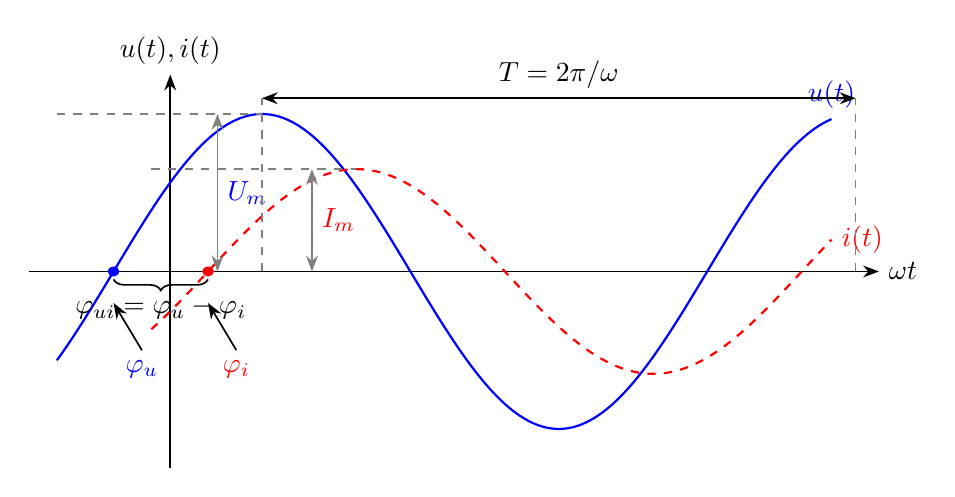
\begin{tikzpicture}[>=Stealth, semithick, xscale=1.2]
    \draw[->] (-1.5,0) -- (7.5,0) node[right] {$\omega t$};
    \draw[->] (0,-2.5) -- (0,2.5) node[above] {$u(t), i(t)$};
    \draw[domain=-1.2:7, samples=200, blue, thick] plot (\x, {2*sin(deg(\x + 0.6))}) node[above] {$u(t)$};
    \draw[domain=-0.2:7, samples=200, red, dashed, thick] plot (\x, {1.3*sin(deg(\x - 0.4))}) node[right] {$i(t)$};
    
    \draw[dashed, gray] (-1.2, 2) -- (0.97, 2);
    \draw[<->, gray] (0.5, 0) -- (0.5, 2) node[midway, right, blue] {$U_m$};
    \draw[dashed, gray] (-0.2, 1.3) -- (1.97, 1.3);
    \draw[<->, gray] (1.5, 0) -- (1.5, 1.3) node[midway, right, red] {$I_m$};
    
    \draw[<->, black] (0.97, 2.2) -- ({0.97 + 2*pi}, 2.2) node[midway, above] {$T = 2\pi/\omega$};
    \draw[dashed, gray] ({0.97 + 2*pi}, 0) -- ({0.97 + 2*pi}, 2.2);
    \draw[dashed, gray] (0.97, 0) -- (0.97, 2.2);
    
    \filldraw[blue] (-0.6, 0) circle (1.5pt);
    \draw[<-] (-0.6, -0.4) -- (-0.3, -1) node[below, blue] {$\varphi_u$};
    \filldraw[red] (0.4, 0) circle (1.5pt);
    \draw[<-] (0.4, -0.4) -- (0.7, -1) node[below, red] {$\varphi_i$};
    
    \draw[decorate, decoration={brace, amplitude=4pt, mirror}] (-0.6, -0.1) -- (0.4, -0.1) node[midway, below=3pt] {$\varphi_{ui} = \varphi_u - \varphi_i$};
\end{tikzpicture}
\end{document}
